\chapter{Software Educacional}
A grande preocupação com o aumento da obesidade infantil fez com que se tornasse
urgente o desenvolvimento de uma referência de crescimento única para a
avaliação de crianças em idade escolar e adolescentes (5 a 19 anos).
Para essa avaliação, o \emph{Center for Disease Control} (CDC) criou um gráfico
que representa o índice de massa corporal (IMC) dentro de uma faixa percentil.

(1) O IMC é um número calculado a partir do peso e altura do indivíduo. É um
indicador confiável de gordura corporal, porém, para crianças e adolescentes, o
IMC leva em consideração também o sexo e a idade, já que nessa fase a quantidade
de gordura corporal varia conforme essas características também.

Conforme indicam Castagni e Menta (2010) apresentar ao aluno o conceito de IMC,
explicar que o excesso de peso não é algo puramente estético e os riscos
envolvidos no excesso ou baixo peso, devem constituir como integranter do
componente de saúde. Somando a esta idéia, Oliveira (2010) mosta que este
índice pode ser utilizado com duplo objetivo, conscientizar alunos e familiares
quanto aos perigos da obesidade e ajudar no ensino de expressões algébricas.

    \section{Forma de avaliação}

    Para avaliação do resultado deve ser encontrado o ponto de intersecção entre
    IMC (eixo vertical) e a idade (eixo horizontal) onde se identifica o
    percentil atingido pela criança ou adolescente.

    \begin{table}
        \begin{center}
        \caption{Classificação do IMC}
        \begin{tabular}{cc} \hline
            \textbf{Classificação}  & \textbf{Faixa de percentil}   \\  \hline
            Abaixo do peso          & Inferior a 5\%                \\
            Peso saudável           & Entre 5 e 85\%                \\
            Risco de sobrepeso      & Entre 85 e 97\%               \\
            Sobrepeso               & Acima de 95\%
        \end{tabular}
        \end{center}
    \end{table}

    Existe também a curva padrão de crescimento infantil estabelecida pela OMS
    (Organização Mundial de Saúde) onde os dados estão separados por faixa
    etária e sexo.

    Para avaliação do resultado deve ser encontrado o ponto de intersecção entre
    a altura (eixo vertical, em centímetros) e a idade (eixo horizontal, em
    meses e anos) onde se identifica o percentil atingido pela criança ou
    adolescente.

    \section{Programa para cálculo e classificação do IMC}
    O programa desenvolvido permite ao professor demonstrar como é realizada a
    relação de proporção entre a massa corporal e a estura, definir a
    exponenciação, além de permitir elaborar sobre os conceitos de percentual
    e percentis de uma distribuição.

    Para tal o programa apresenta três áreas complementares:

    \begin{enumerate}

        \item Cadastro da turma \ref{fig:cad_turma}

        \item Cadastro do aluno \ref{fig:cad_aluno}

        \item Cadastro da avaliação \ref{fig:cad_avaliacao}

    \end{enumerate}

        \subsection{Cadastro turma}

        Permite ao professor cadastrar as turmas nas quais são ministradas aulas.

        \begin{figure}[htb]
            \centering
            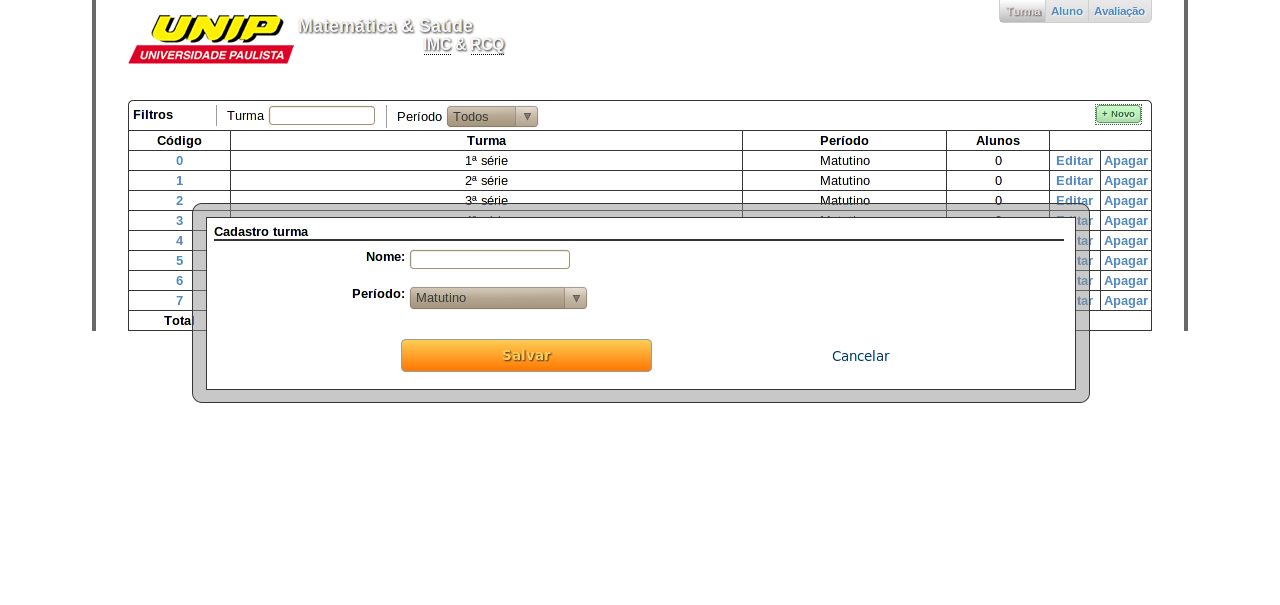
\includegraphics[width=10cm]{programa/media/image/cadastro_turma.png}
            \caption{Cadastro turma}
            \label{fig:cad_turma}
        \end{figure}

        \subsection{Cadastro aluno}

        Nesta seção o docente pode cadastras os alunos de uma determinada turma.

        \begin{figure}[htb]
            \centering
            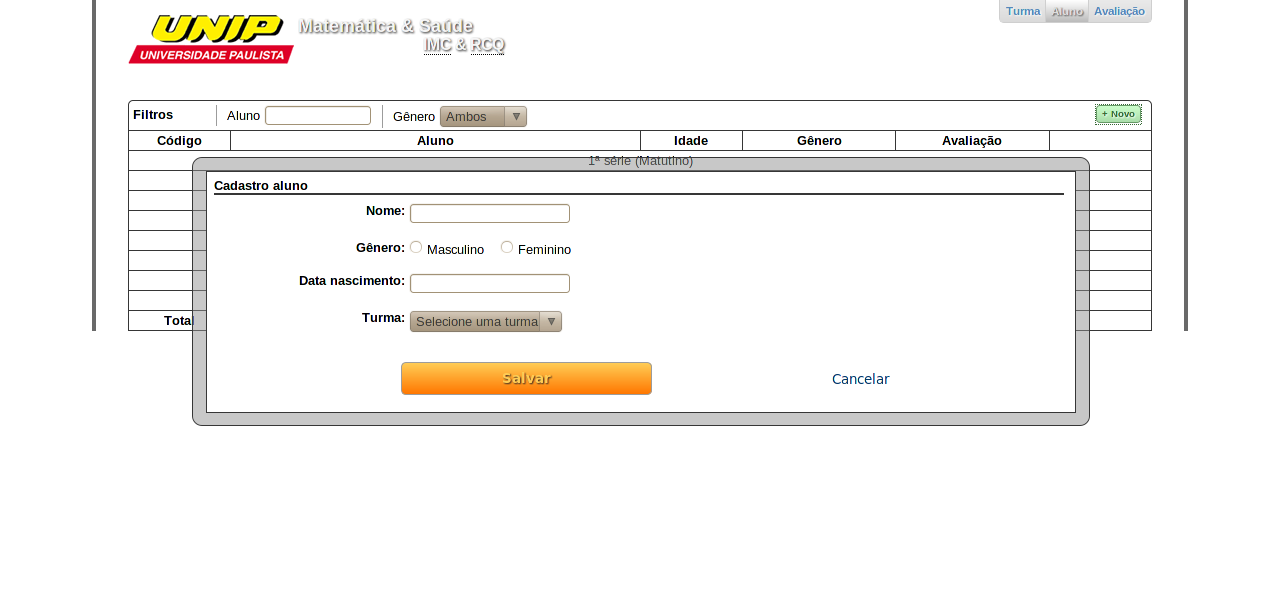
\includegraphics[width=10cm]{programa/media/image/cadastro_aluno.png}
            \caption{Cadastro aluno}
            \label{fig:cad_aluno}
        \end{figure}

        \subsection{Cadastro avaliação}

        Nesta área são cadastrados os detalhes da avaliação, tais como data,
        massa corporal e estatura do aluno.

        Além deste cadastro, nesta seção, cada aluno é classificado quanto ao
        IMC apresentado.

        \begin{figure}[htb]
            \centering
            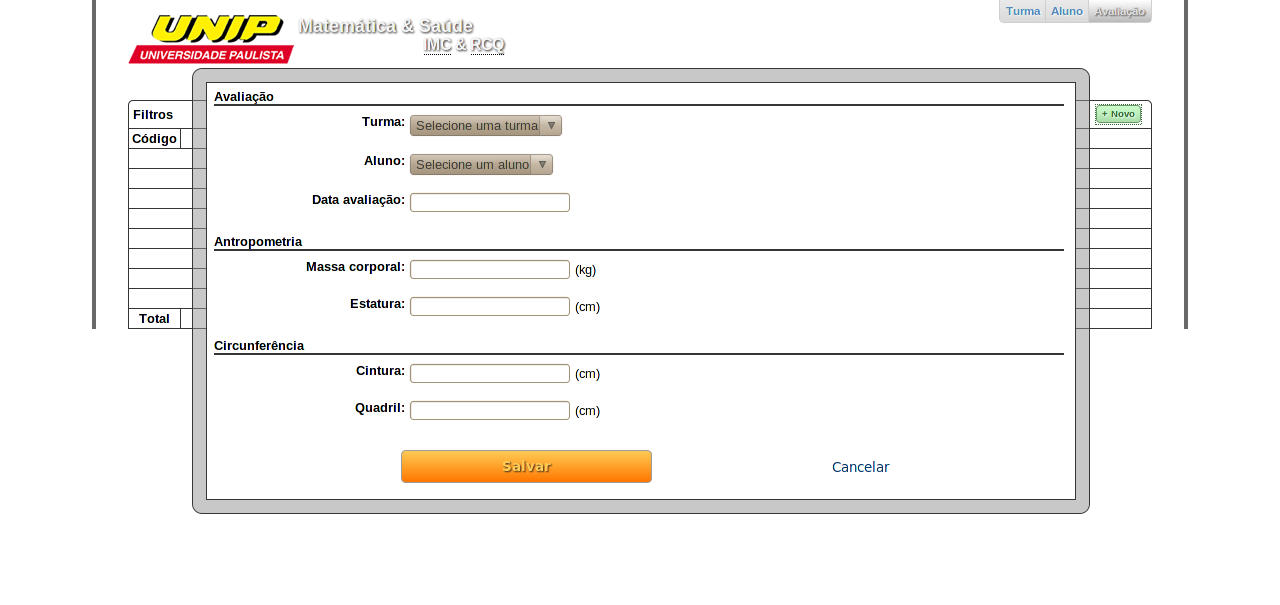
\includegraphics[width=10cm]{programa/media/image/cadastro_avaliacao.png}
            \caption{Cadastro avaliação}
            \label{fig:cad_avaliacao}
        \end{figure}
